%% abtex2-modelo-relatorio-tecnico.tex, v-1.9.6 laurocesar
%% Copyright 2012-2016 by abnTeX2 group at http://www.abntex.net.br/ 
%%
%% This work may be distributed and/or modified under the
%% conditions of the LaTeX Project Public License, either version 1.3
%% of this license or (at your option) any later version.
%% The latest version of this license is in
%%   http://www.latex-project.org/lppl.txt
%% and version 1.3 or later is part of all distributions of LaTeX
%% version 2005/12/01 or later.
%%
%% This work has the LPPL maintenance status `maintained'.
%% 
%% The Current Maintainer of this work is the abnTeX2 team, led
%% by Lauro César Araujo. Further information are available on 
%% http://www.abntex.net.br/
%%
%% This work consists of the files abntex2-modelo-relatorio-tecnico.tex,
%% abntex2-modelo-include-comandos and abntex2-modelo-references.bib
%%

% ------------------------------------------------------------------------
% ------------------------------------------------------------------------
% abnTeX2: Modelo de Relatório Técnico/Acadêmico em conformidade com 
% ABNT NBR 10719:2015 Informação e documentação - Relatório técnico e/ou
% científico - Apresentação
% ------------------------------------------------------------------------ 
% ------------------------------------------------------------------------

\documentclass[
	% -- opções da classe memoir --
	12pt,				% tamanho da fonte
	openright,			% capítulos começam em pág ímpar (insere página vazia caso preciso)
	%twoside,			% para impressão em recto e verso. Oposto a oneside
	a4paper,			% tamanho do papel. 
	% -- opções da classe abntex2 --
	%chapter=TITLE,		% títulos de capítulos convertidos em letras maiúsculas
	%section=TITLE,		% títulos de seções convertidos em letras maiúsculas
	%subsection=TITLE,	% títulos de subseções convertidos em letras maiúsculas
	%subsubsection=TITLE,% títulos de subsubseções convertidos em letras maiúsculas
	% -- opções do pacote babel --
	english,			% idioma adicional para hifenização
	french,				% idioma adicional para hifenização
	spanish,			% idioma adicional para hifenização
	brazil,				% o último idioma é o principal do documento
	]{abntex2}



% PACOTES

% ---
% Pacotes fundamentais 
\usepackage{lmodern}			% Usa a fonte Latin Modern
\usepackage[T1]{fontenc}		% Selecao de codigos de fonte.
\usepackage[utf8]{inputenc}		% Codificacao do documento (conversão automática dos acentos)
\usepackage{indentfirst}		% Indenta o primeiro parágrafo de cada seção.
\usepackage{color}				% Controle das cores
\usepackage{graphicx}			% Inclusão de gráficos
\usepackage{microtype} 			% para melhorias de justificação
% ---

% Pacotes adicionais, usados no anexo do modelo de folha de identificação
\usepackage{multicol}
\usepackage{multirow}

\usepackage{float} % para utilizar o H de tabelas e figuras e mante-las no lugar
% ---

%----------------- PARA INSERIR ARQUIVOS DE CODIGOS -----------------%
\usepackage{xcolor}
% Definindo novas cores
\definecolor{verde}{rgb}{0,0.5,0}
% Configurando layout para mostrar codigos C++
\usepackage{listings}
\lstset{
  language=Verilog, %indicar a linguagem utilizada
  basicstyle=\ttfamily\tiny, 
  keywordstyle=\color{blue}, 
  stringstyle=\color{verde}, 
  commentstyle=\color{gray}, 
  extendedchars=true, 
  showspaces=false, 
  showstringspaces=false, 
  numbers=left,
  numberstyle=\tiny,
  breaklines=true, 
  backgroundcolor=\color{green!10},
  breakautoindent=true, 
  captionpos=b,
  xleftmargin=0pt,
}
% -----------------% FIM INSERIR ARQUIVOs DE CODIGO -----------------%

% Pacotes de citações
\usepackage[brazilian,hyperpageref]{backref}	 % Paginas com as citações na bibl
\usepackage[num]{abntex2cite}	% Citações padrão ABNT
\citebrackets() %citação numérica entre colchetes
% --- 


% CONFIGURAÇÕES DE PACOTES

% Configurações do pacote backref
% Usado sem a opção hyperpageref de backref
\renewcommand{\backrefpagesname}{Citado na(s) página(s):~}
% Texto padrão antes do número das páginas
\renewcommand{\backref}{}
% Define os textos da citação
\renewcommand*{\backrefalt}[4]{
	\ifcase #1 %
		Nenhuma citação no texto.%
	\or
		Citado na página #2.%
	\else
		Citado #1 vezes nas páginas #2.%
	\fi}%
% ---


% Informações de dados para CAPA e FOLHA DE ROSTO
\titulo{Desenvolvimento de Sistemas Computacionais
\\Laboratório de Arquitetura de Computadores }
\autor{ID: .......} %NAO PREENCHER
\local{São José dos Campos - Brasil}
\data{Abril de 2017}
\instituicao{
  Docente: Prof. Dr. Tiago de Oliveira
  \par
  Universidade Federal de São Paulo - UNIFESP
  \par
  Instituto de Ciência e Tecnologia - Campus São José dos Campos
}
\tipotrabalho{Relatório técnico}
\preambulo{Relatório apresentado à Universidade Federal de São Paulo como parte dos requisitos para aprovação na disciplina de Laboratório de Sistemas Computacionais: Arquitetura e Organização de Computadores.}
% ---

% Configurações de aparência do PDF final

% alterando o aspecto da cor azul
\definecolor{blue}{RGB}{41,5,195}

% informações do PDF
\makeatletter
\hypersetup{
     	%pagebackref=true,
		pdftitle={\@title}, 
		pdfauthor={\@author},
    	pdfsubject={\imprimirpreambulo},
	    pdfcreator={LaTeX with abnTeX2},
		pdfkeywords={abnt}{latex}{abntex}{abntex2}{relatório técnico}, 
		colorlinks=true,       		% false: boxed links; true: colored links
    	linkcolor=blue,          	% color of internal links
    	citecolor=blue,        		% color of links to bibliography
    	filecolor=magenta,      		% color of file links
		urlcolor=blue,
		bookmarksdepth=4
}
\makeatother
% --- 


% Espaçamentos entre linhas e parágrafos 

% O tamanho do parágrafo é dado por:
\setlength{\parindent}{1.3cm}

% Controle do espaçamento entre um parágrafo e outro:
\setlength{\parskip}{0.2cm}  % tente também \onelineskip

% compila o indice
\makeindex
% ---



% ------------------------------------------------
% Início do documento
\begin{document}

% Seleciona o idioma do documento (conforme pacotes do babel)
%\selectlanguage{english}
\selectlanguage{brazil}

% Retira espaço extra obsoleto entre as frases.
\frenchspacing 

% ----------------------------------------------------------
% ELEMENTOS PRÉ-TEXTUAIS
% ----------------------------------------------------------
% \pretextual

% ---
% Capa
\imprimircapa
% ---

% ---
% Folha de rosto
\imprimirfolhaderosto*
% ---

% ---
% RESUMO
% resumo na língua vernácula (obrigatório)
\setlength{\absparsep}{18pt} % ajusta o espaçamento dos parágrafos do resumo
\begin{resumo}
 Segundo a NBR6028:2003 \cite{NBR6028:2003}, o resumo deve ressaltar o
 objetivo, o método, os resultados e as conclusões do documento. A ordem e a extensão
 destes itens dependem do tipo de resumo (informativo ou indicativo) e do
 tratamento que cada item recebe no documento original. O resumo deve ser
 precedido da referência do documento, com exceção do resumo inserido no
 próprio documento. (\ldots) As palavras-chave devem figurar logo abaixo do
 resumo, antecedidas da expressão Palavras-chave:, separadas entre si por
 ponto e finalizadas também por ponto. Palavras estrangeiras devem estar em destaque como em \emph{Hardware}

 \noindent
 \textbf{Palavras-chaves}: latex. abntex. editoração de texto.
\end{resumo}

%------LISTAS SÃO OPCIONAIS---------
% inserir lista de ilustrações
\pdfbookmark[0]{\listfigurename}{lof}
\listoffigures*
\clearpage

% inserir lista de tabelas
\pdfbookmark[0]{\listtablename}{lot}
\listoftables*
\clearpage
% ---

%SUMÁRIO É OBRIGATÓRIO
% inserir o sumario
\pdfbookmark[0]{\contentsname}{toc}
\tableofcontents*
% ---


% ----------------------------------------------------------
% ELEMENTOS TEXTUAIS
\textual

% ----------------------------------------------------------
\chapter{Introdução}
Palavras estrangeiras como \emph{hardware} devem ser destacadas.

%------------------- MODELO DE FIGURA -----------------------------
Modelo da \autoref{fig:esquematico}:
\begin{figure}[H]
\centering 
\caption{Esquematico} \label{fig:esquematico}
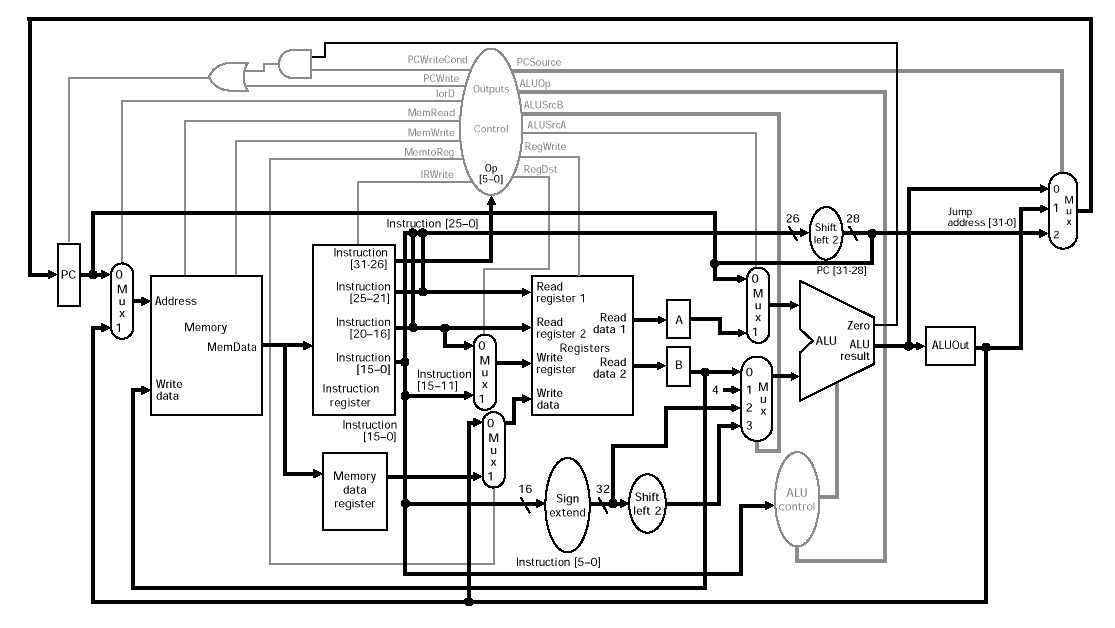
\includegraphics[scale=0.3]{esquematico.png}
\legend{Fonte: Computer Organization and Design \cite{patterson2007} }
\end{figure}


%------------------- MODELO DE TABELA -----------------------------
Modelo da \autoref{tab:Instr3OP}:
\begin{table}[htb]
\centering
\ABNTEXfontereduzida
\caption{Exemplo de um formato de Instruções} \label{tab:Instr3OP}
\begin{tabular}{r|p{2cm}|p{1.7cm}|p{1.7cm}|p{1.7cm}|p{3cm}} 
\textbf{Tamanho (bits)} & 6 & 5 & 5 & 5 & 11 \\ \hline
\textbf{Campo} & OPcode & Reg1 & Reg2 & Reg3 & Blank \\ \hline
\textbf{Bits} & 31 - 26 & 25 - 21 & 20 - 16 & 15 - 11 & 10 - 0\\
\end{tabular}
\legend{Fonte: O Autor}
\end{table}

Como utilizar \textbf{Anexos}
Material que não seja de autoria própria que traga maiores detalhes de algo utilizado no decorrer do relatório

Como utilizar \textbf{Apêndices}
Material de autoria própria que traga maiores detalhes e que não seja essencial no decorrer do relatório.

Modos de comandos $\backslash$ref\\
$\backslash$ref: \ref{fig:esquematico}\\
$\backslash$nameref: \nameref{fig:esquematico}\\
$\backslash$autoref: \autoref{fig:esquematico}\\

Existe uma forma de inserir arquivos de códigos diretamente no latex, verificar a formatação nas linhas 70 a 93 do código latex e a inserção feita do código \nameref{code:BinToBCD2.v} no \autoref{code:BinToBCD2.v} 

\chapter[Objetivos]{Objetivos}
\section{Geral}
Descrever o objetivo geral do projeto
\section{Específico}
Descrever com detalhes os objetivos da etapa atual.

\chapter{Fundamentação Teórica}


\chapter{Desenvolvimento}


\chapter{Resultados Obtidos e Discussões}


\chapter{Considerações Finais}



% ---
% Finaliza a parte no bookmark do PDF
% para que se inicie o bookmark na raiz
% e adiciona espaço de parte no Sumário
% ---
\phantompart


% ----------------------------------------------------------
% ELEMENTOS PÓS-TEXTUAIS
% ----------------------------------------------------------
\postextual

% ----------------------------------------------------------
% Referências bibliográficas
% ----------------------------------------------------------
\bibliography{referencias}


% ----------------------------------------------------------
% Apêndices
% ----------------------------------------------------------

% ---
% Inicia os apêndices
% ---
\begin{apendicesenv}

% Imprime uma página indicando o início dos apêndices
\partapendices

% ----------------------------------------------------------
\chapter{BinToBCD2.v}
\label{code:BinToBCD2.v}
Código do arquivo BinToBCD2.v
\lstinputlisting{Codigos/BinToBCD2.v} 
% ----------------------------------------------------------

% ----------------------------------------------------------
\chapter{Apêndice 2}
% ----------------------------------------------------------


\end{apendicesenv}
% ---


% ----------------------------------------------------------
% Anexos
% ----------------------------------------------------------

% ---
% Inicia os anexos
% ---
\begin{anexosenv}

% Imprime uma página indicando o início dos anexos
\partanexos

% ---
\chapter{Anexo 1}
% ---

% ---
\chapter{Anexo 2}
% ---

\end{anexosenv}

%---------------------------------------------------------------------
% INDICE REMISSIVO
%---------------------------------------------------------------------

\phantompart

\printindex


\end{document}
